\clearpage
\chapter{Study Guide 1}

\section{Vectors}
\horizontalline{0}{0}

\begin{center}
    \large{\textbf{Study Guide Instructions}}
\end{center}

\horizontalline{-1}{0}

\begin{itemize}
    \item Submit your work in Gradescope as a PDF - you will identify where your “questions are.”
    \item Identify the question number as you submit.  Since we grade "blind" if the questions are NOT identified, the work WILL NOT BE GRADED and a 0 will be recorded. Always leave enough time to 
    identify the questions when submitting.
    \item One section per page (if a page or less) - We prefer to grade the main solution in a single page, extra work can be included on the following page.
    \item Long instructions may be removed to fit on a single page.
    \item \textbf{Do not start a new question in the middle of a page.}
    \item Solutions to book questions are provided for reference.
    \item You may NOT submit given solutions - this includes minor modifications - as your own.
    \item Solutions that do not show individual engagement with the solutions will be marked as no credit and can be considered a violation of honor code.
    \item If you use the given solutions you must reference or explain how you used them, in particular...
\end{itemize}

\horizontalline{-1}{0}

\begin{center}
    \large{\textbf{Method Selection}}
\end{center}

\horizontalline{-1}{0}

\textbf{For full credit,  EACH book exercise in the Study Guides must use one or more of the following methods and FOR EACH QUESTION.  Identify the number the method by number to ensure full credit.}

\begin{itemize}
    \item \textbf{Method 1} - Provide original examples which demonstrate the ideas of the exercise in addition to your solution.
    \item \textbf{Method 2} - Include and discuss the specific topics needed from the chapter and how they relate to the question.
    \item \textbf{Method 3} - Include original Python code, of reasonable length (as screenshot r text)  to show how the topic or concept was explored.
    \item \textbf{Method 4} - Expand the given solution in a significant way, with additional steps and comments. All steps are justified. This is a good method for a proof for which you are only given a basic outline.
    \item \textbf{Method 5} - Attempt the exercise without looking at the solution and then the solution is used to check work. Words are used to describe the results.
    \item \textbf{Method 6} - Provide an analysis of the strategies used to understand the exercise, describing in detail what was challenging, who helped you or what resources were used. The process of understanding is
    described.
\end{itemize}

% Problem 1
\begin{problem}{Problem 1}
    \begin{statement}{Problem Description}
        Reading the book carefully is essential in this class and in all advanced mathematics. This is an exercise in annotation.

        For this first exercise, pick a section or page from Chapter one of VMLS. \vspace*{1em}

        Read straight through the section once for an overview. Include the following 3 items for \#1.

        \begin{enumerate}[label=(\alph*)]
            \item Write down your initial thoughts, questions, and first impressions (‘whaaat???’)
            \item Now, return to the section and slowly work through each line using a pencil or pen.
            \begin{itemize}
                \item Expand equations.
                \item Identify key concepts and explain in your own words.
                \item Make note - is that a vector or a scalar?
                \item Fill in missing ideas or steps.
                \item Include a screenshot of your annotation.
            \end{itemize}
            \item How has your understanding of the section changed?
        \end{enumerate}
    \end{statement}

    
    \begin{Highlight}[Solution - Part (a)]
        For this problem, I am going to utilize \textbf{Method 2}. \vspace*{1em}

        For this part of the problem, I will be reviewing \textbf{VMLS Page 19}, particularly the part about the inner product definition.

        To begin, this page in the textbook gives a definition of what a inner product (dot or scalar product) is. This operation takes two vectors of equal length and `multiplies' them together
        to get a scalar value. 
        
        Another way that an inner product is defined is with the use of the vectors magnitude and angle in between the vectors. If we let $A$ and $B$ represent the magnitudes of vectors $a$ and $b$ 
        respectively and $\theta$ represent the angle in between these vectors, the dot product of two vectors can be defined as

        \setcounter{equation}{0}
        \begin{equation}
            a \cdot b = AB\cos{(\theta)}.
        \end{equation}

        My initial thoughts after reading this section was that this section skipped a lot of math in its definitions (as expected when talking about mathematical text books) and it could be very 
        confusing to readers who do not have a more in depth mathematical background. With this being said, I did not know about some of the properties that were mentioned in this section. I also 
        think this section of the textbook does not give an in depth explanation of what the transpose of a matrix is (vectors are indeed matrices) and that can also be confusing as to what that means.
    \end{Highlight}

    \begin{Highlight}[Solution - Part (b)]
        For this problem, I am going to utilize \textbf{Method 2}. \vspace*{1em}

        I first want to begin with a more clear definition of what the transpose of a matrix is. In short, the transpose of a matrix takes the rows of matrix, beginning from the first row and takes the
        elements in those rows and puts them in the column of a matrix. The easiest example of this can be seen with an arbitrary $2 \times 2$ matrix. Lets say we have a matrix $A$, the transpose of this
        matrix (denoted as $A^{T}$) is then

        \begin{equation}
            A = 
            \begin{bmatrix}
                a & b \\
                c & d \\
            \end{bmatrix}
            \implies
            A^{T} = 
            \begin{bmatrix}
                a & c \\
                b & d \\
            \end{bmatrix}.
        \end{equation}
        Because of the simple nature of a $2 \times 2$ matrix, it may just seem that we are switching diagonal elements in a matrix. That is not the case when we are working with larger matrices.

        If we now expand the definition of the transpose of a matrix in equation (2) to a vector, we can see that a vector of length three's transpose (the vector is denoted as $a$) is then

        \begin{equation}
            a = 
            \begin{bmatrix}
                a \\
                b \\
                c \\
            \end{bmatrix}
            \implies
            a^{T} = 
            \begin{bmatrix}
                a & b & c \\
            \end{bmatrix}.
        \end{equation}
        The nature of which matrix multiplication occurs is that of `row times column'. The necessity for why we have to transpose a vector in order to take the inner product of said vector with
        another vector is that one vector must be a row vector and the other must be a column vector.

        If we take a further look at matrix multiplication, it can possibly help us understand the inner product a little bit more. Say we have two matrices $(A)$ and $(B)$, in general these matrices
        are

        \begin{equation}
            A = 
            \begin{bmatrix}
                a & b \\
                c & d \\
            \end{bmatrix}
            \hspace*{5pt}
            B = 
            \begin{bmatrix}
                e & f \\
                g & h \\
            \end{bmatrix}.
        \end{equation}
        If we now multiply the matrices found in equation (4), we will have

        \begin{equation}
            A \times B =
            \begin{bmatrix}
                a & b \\
                c & d \\
            \end{bmatrix}
            \times
            \begin{bmatrix}
                e & f \\
                g & h \\
            \end{bmatrix}
            = 
            \begin{bmatrix}
                a(e) + b(g) & a(f) + b(h) \\
                c(e) + d(g) & c(f) + d(h) \\
            \end{bmatrix}.
        \end{equation}
        Now, we can observe that each element in the resulting matrix is indeed a scalar value. In the context of vectors, we do not get a vector (or matrix) as the resulting value that comes from
        an inner product, we get a scalar value. This is because when we take an inner product of two vectors, we are performing matrix multiplication of a $(1 \times n)$ matrix with that of a 
        $(n \times 1)$ matrix.

        This means, a better way to define the inner product of two vectors would then look something like

        \begin{equation}
            a = 
            \begin{bmatrix}
                a_{1} \\
                a_{2} \\
                \vdots \\
                a_{n} \\
            \end{bmatrix}
            \hspace*{5pt}
            b = 
            \begin{bmatrix}
                b_{1} \\
                b_{2} \\
                \vdots \\
                b_{n} \\
            \end{bmatrix}
            \implies
            a \cdot b =
            a^{T}b = 
            \begin{bmatrix}
                a_{1} & a_{2} & \dots & a_{n} \\
            \end{bmatrix}
            \times
            \begin{bmatrix}
                b_{1} \\
                b_{2} \\
                \vdots \\
                b_{n} \\
            \end{bmatrix}
            = a_{1}b_{1} + a_{2}b_{2} + \dots + a_{n}b_{n}.
        \end{equation}
        Equation (6) in my eyes gives a more in depth explanation of the inner product and how it is calculated. Filling in these gaps for how to carry out these calculations can be very beneficial
        to understanding more general or complicated examples of the same topic.

        Now I would like to discuss the properties of inner products. The first property that we encounter is the \textbf{\textit{commutativity}} property. We can do a pseudo proof of this property

        \begin{equation}
            a = 
            \begin{bmatrix}
                a_{1} \\
                a_{2} \\
            \end{bmatrix}
            \hspace*{5pt}
            b = 
            \begin{bmatrix}
                b_{1} \\
                b_{2} \\
            \end{bmatrix}
            \implies
            a \cdot b = a^{T}b =
            \begin{bmatrix}
                a_{1} & a_{2} \\
            \end{bmatrix}
            \times
            \begin{bmatrix}
                b_{1} \\
                b_{2} \\
            \end{bmatrix}
            = a_{1}(b_{1}) + a_{2}(b_{2}),
        \end{equation}
        where now we do the reverse

        \begin{equation}
            b \cdot a = b^{T}a =
            \begin{bmatrix}
                b_{1} & b_{2} \\
            \end{bmatrix}
            \times
            \begin{bmatrix}
                a_{1} \\
                a_{2} \\
            \end{bmatrix}
            = b_{1}(a_{1}) + b_{2}(a_{2}).
        \end{equation}
        Because of the commutativity property of real numbers we can say $a_{1}(b_{1}) = b_{1}(a_{1})$ and vice versa to further say
        
        \begin{equation}
            a_{1}(b_{1}) + a_{2}(b_{2}) = b_{1}(a_{1}) + b_{2}(a_{2})
            \implies
            a^{T}b = b^{T}a.
        \end{equation}

        We now move on to \textbf{\textit{associativity with scalar multiplication}}. Starting with the same vectors defined in equation (7) we can do another pseudo proof of this property

        \begin{equation}
            (\gamma a^{T})b = \gamma
            \begin{bmatrix}
                a_{1} & a_{2} \\
            \end{bmatrix}
            \times
            \begin{bmatrix}
                b_{1} \\
                b_{2} \\
            \end{bmatrix}
            = 
            \begin{bmatrix}
                \gamma(a_{1}) & \gamma(a_{2}) \\
            \end{bmatrix}
            \times
            \begin{bmatrix}
                b_{1} \\
                b_{2} \\
            \end{bmatrix}
            = \gamma(a_{1})b_{1} + \gamma(a_{2})b_{2}
        \end{equation}
        where we can then do

        \begin{equation}
            \gamma(a^{T}b) = \gamma \Bigg(
            \begin{bmatrix}
                a_{1} & a_{2} \\
            \end{bmatrix}
            \times
            \begin{bmatrix}
                b_{1} \\
                b_{2} \\
            \end{bmatrix}
            \Bigg) = \gamma (a_{1}(b_{1}) + a_{2}(b_{2})) = \gamma a_{1}(b_{1}) + \gamma a_{2}(b_{2}) \implies (\gamma a^{T})b = \gamma(a^{T}b).
        \end{equation}
        Equations (10) and (11) are thus equivalent as their only differences lie in the formatting of the multiplication of the elements.

        We now move on to our last property shown on this page, the \textbf{\textit{distributivity with vector addition}} property. We first start with three vectors

        \begin{equation}
            a = 
            \begin{bmatrix}
                a_{1} \\
                a_{2} \\
            \end{bmatrix}
            \hspace*{5pt}
            b = 
            \begin{bmatrix}
                b_{1} \\
                b_{2} \\
            \end{bmatrix}
            \hspace*{5pt}
            c = 
            \begin{bmatrix}
                c_{1} \\
                c_{2} \\
            \end{bmatrix}.
        \end{equation}
        We then first show

        \begin{align}
            (a + b)^{T}c = & \Bigg(
            \begin{bmatrix}
                a_{1} \\
                a_{2} \\
            \end{bmatrix}
            + 
            \begin{bmatrix}
                b_{1} \\
                b_{2} \\
            \end{bmatrix}
            \Bigg)^{T} \times
            \begin{bmatrix}
                c_{1} \\
                c_{2} \\
            \end{bmatrix}
            = \Bigg(
            \begin{bmatrix}
                a_{1} + b_{1} \\
                a_{2} + b_{2} \\
            \end{bmatrix}
            \Bigg)^{T} \times
            \begin{bmatrix}
                c_{1} \\
                c_{2} \\
            \end{bmatrix}
            = 
            \begin{bmatrix}
                a_{1} + b_{1} & a_{2} + b_{2} \\
            \end{bmatrix}
            \times 
            \begin{bmatrix}
                c_{1} \\
                c_{2} \\
            \end{bmatrix} \\
            = & (a_{1} + b_{1})c_{1} + (a_{2} + b_{2})c_{2} = a_{1}(c_{1}) + b_{1}(c_{1}) + a_{2}(c_{2}) + b_{2}(c_{2}).
        \end{align}
        We can now go on to show that the result from equation (14) is equal to

        \begin{align}
            a^{T}c + b^{T}c = &
            \begin{bmatrix}
                a_{1} \\
                a_{2} \\
            \end{bmatrix}^{T}
            \times 
            \begin{bmatrix}
                c_{1} \\
                c_{2} \\
            \end{bmatrix}
            + 
            \begin{bmatrix}
                b_{1} \\
                b_{2} \\
            \end{bmatrix}^{T}
            \times
            \begin{bmatrix}
                c_{1} \\
                c_{2} \\
            \end{bmatrix}
            =
            \begin{bmatrix}
                a_{1} & a_{2} \\
            \end{bmatrix}
            \times
            \begin{bmatrix}
                c_{1} \\
                c_{2} \\
            \end{bmatrix}
            +
            \begin{bmatrix}
                b_{1} & b_{2} \\
            \end{bmatrix}
            \times
            \begin{bmatrix}
                c_{1} \\
                c_{2} \\
            \end{bmatrix} \\
            = & a_{1}(c_{1}) + a_{2}(c_{2}) + b_{1}(c_{1}) + b_{2}(c_{2}).
        \end{align}
        Using the commutativity property of addition we can then say

        \begin{equation}
            (a + b)^{T}c = a^{T}c + b^{T}c
        \end{equation}
        and thus the property has been proved.
    \end{Highlight}

    \begin{Highlight}[Solution - Part (c)]
        Before reading this section, I did not know of the properties that pertained to the inner product. Such as the commutativity property. After reading this chapter I gained a lot of insight
        into these other properties and how they can be applied to vectors. From my prior experience to linear algebra, I had a good understanding of the inner product but I didn't really know of
        these properties all too well. These properties can be utilized in certain scenarios to make problems easier and it has provided me some more tools that I can possibly use in the future.
    \end{Highlight}
\end{problem}

% Problem 1 Summary
\begin{summary}{Problem 1 Summary}
    \begin{statement}{Procedure}
        \begin{itemize}
            \item This problem encapsulates summarizing a section / page of a textbook and highlighting important aspects from the chapter
        \end{itemize}
    \end{statement}
    \begin{statement}{Key Concepts}
        \begin{itemize}
            \item Important aspects from this section are what an inner product is and how a transpose works on a matrix
            \item Inner products are commutative, associative, and distributive
        \end{itemize}
    \end{statement}
    \begin{statement}{Variations}
        \begin{itemize}
            \item This particular example doesn't have much variations since it is annotating a chapter from the textbook
        \end{itemize}
    \end{statement}
\end{summary}

% Problem 2
\begin{problem}{Problem 2}
    \begin{statement}{Problem Description}
        Solve the Random exercise from the video and Piazza in your own words here. \vspace*{1em}

        Symptoms vector. A 20-vector $s$ records whether each of 20 different symptoms is present in a medical patient, with $s_i = 1$ meaning the patient has the symptom and $s_i = 0$ meaning she does not. Express the following 
        using vector notation. \vspace*{1em}

        \textbf{Original Questions}

        \begin{enumerate}[label=(\alph*)]
            \item The total number of symptoms the patient has.
            \item The patient exhibits five out of the first ten symptoms.
        \end{enumerate}
    \end{statement}

    \begin{Highlight}[Solution - Part (a)]
        For this solution, I a going utilize \textbf{Method 5} for this problem. \vspace*{1em}

        The vector $S$ encapsulates the symptoms that a patient is showing. Inside this vector, a given index is denoted with a 1 if they have the symptom and a 0 if they do not have the symptom. To accurately count the number of
        symptoms that a patient has, we must take the inner product of the symptoms vector $S$ with the the unit vector \textbf{1}. Let $\sigma$ denote the total number of symptoms that a patient has. Mathematically this will look like

        \setcounter{equation}{0}
        \begin{equation}
            \sigma = \sum_{i} S_{i}\mathbf{1}_{i} = S^{T}\mathbf{1}.
        \end{equation}

        The solution found in one can be explained further by looking at this simple example. For simplicity, I will simplify our vector down to only length 3.

        \begin{equation}
            \sigma = \sum_{i} S_{i}\mathbf{1}_{i} = S^{T}\mathbf{1} = 
            \begin{pmatrix}
                1 \\
                0 \\
                1 \\
            \end{pmatrix}^{T}
            \cdot
            \begin{pmatrix}
                1 \\
                1 \\
                1 \\
            \end{pmatrix}
            =
            \begin{pmatrix}
                1 & 0 & 1 \\
            \end{pmatrix}
            \cdot
            \begin{pmatrix}
                1 \\
                1 \\
                1 \\
            \end{pmatrix}
            = 1(1) + 0(1) + 1(1) = 1 + 0 + 1 = 2.
        \end{equation}
        In the case of equation (2), we see that there are a max of 3 possible symptoms and the current patient only has 2 symptoms. The unit vector \textbf{1} helps
        accurately count the number of symptoms that a patient possesses because when the inner product of the two matrices are taken, if a patient is not showing a symptom
        then the multiplication between the symptom and unit vector's for the given index that represents that symptom will be zero. In the example of (2) above, we see that
        the patient is only showing signs for symptom 1 and 3. This in turn means when the calculation is carried out the patient will only come back with showing 2 symptoms.

        For brevity's sake, I simplified the problem as shown in equation (2) to be that of only three possible symptoms. This specific scenario can be generalized to meet 
        any arbitrary number of symptoms that a patient may have. In our case, the patient may show up to 20 possible symptoms. The general case for the number of possible 
        symptoms can be seen in equation (1) above.
    \end{Highlight}

    \begin{Highlight}[Solution - Part (b)]
        For this solution, I a going utilize \textbf{Method 5} for this problem. \vspace*{1em}

        If a patient is showing five out of the first ten symptoms, this means the values for $S$ in the range of indices 1 to 10 must either be zero or one. But the total number
        of symptoms (1's) that show up in the first ten possible symptoms ($S_{1:10}$) must add up to be 5. In general, the number of possible combinations for these can be calculated.
        In our case, for the patient is showing 5 out of the first 10 symptoms. The total number of combinations is

        \begin{equation}
            C(10,5) = 
            \begin{pmatrix}
                10 \\
                5 \\
            \end{pmatrix}
            = \frac{10!}{5!(10-5)!} = \frac{10\cdot9\cdot8\cdot7\cdot6}{5\cdot4\cdot3\cdot2\cdot1} = 252.
        \end{equation}

        Since I would be spending the rest of the semester creating all of these possible combinations, we can generalize this scenario. Let $\bar{S}$ represent one of the 252 possible
        combinations of a patient showing 5 out of the first 10 symptoms where the values of $S_{11:20}$ are zero. This in turn means that we can generalize equation (1) to now be

        \begin{equation}
            \sigma = \sum_{i} \bar{S_{i}}\mathbf{1_{i}} = \bar{S}^{T}\mathbf{1} = 5
        \end{equation}

        Further more, if we generalize equation (4) to encapsulate all 252 combinations, we now have

        \begin{equation}
            \sum_{j}\sum_{i} \bar{S_{j}}_{i}\mathbf{1} = \sum_{j} \bar{S}^{T}_{j}\mathbf{1}.
        \end{equation}

        Here, $j$ represents one of the 252 combinations for how a patient can have 5 out of the first 10 symptoms and $i$ represents the index of that given index of that particular vector
        $j$. The resulting value of equation (4) will always be 5.
    \end{Highlight}

    \begin{Highlight}[Comparison To Solution]
        The answer that I arrived to for part (a) of this problem is identical to that of the one in the solution manual and the one that is in the video on Moodle.

        For the answer to part (b), I feel like the solution manual is missing the fact that there are a number of potential possibilities that can represent the vector $a$ that they have
        in the solution manual. I feel like my solution to this problem is more general in that I have taken into account the number of possibilities there are for a patient showing 5 of
        the first 10 symptoms that are possible. In comparing my solution to that of the solution manual, we had the same answer for the other 10 symptoms ($S_{11:20}$) in that they were
        all zero.
    \end{Highlight}
\end{problem}

% Problem 2
\begin{summary}{Problem 2 Summary}
    \begin{statement}{Procedure}
        \begin{enumerate}[label = (\alph*)]
            \item Part (a)
            \begin{itemize}
                \item Create a variable that represents the number of symptoms that a patient is currently showing with the use of the \textbf{1} vector and a boolean vector that represents the symptom(s)
                that a current patient is exhibiting
                \item Take the inner product between these two vectors to count the number of symptoms that someone is currently showing
                \item Because $S$ is a boolean vector, any symptom that a patient is not showing will have a 0 for that element
            \end{itemize}
            \item Part (b)
            \begin{itemize}
                \item Because there are 252 possibilities for this answer, we represent all possibilities for a patient showing 5 out of the first 10 symptoms with 
                \begin{equation*}
                    \sum_{j}\sum_{i} \bar{S_{j}}_{i}\mathbf{1} = \sum_{j} \bar{S}^{T}_{j}\mathbf{1}.
                \end{equation*}
                This expression will sum over each possibility of a patient showing 5 out of the first 10 symptoms.
            \end{itemize}
        \end{enumerate}
    \end{statement}
    \begin{statement}{Key Concepts}
        \begin{enumerate}[label = (\alph*)]
            \item Part (a)
            \begin{itemize}
                \item This part of the problem is showing how a scalar value can be constructed with the use of two vectors
                \item We use a boolean vector to resemble if someone is showing a symptom and the \textbf{1} vector to represent all of the 20 symptoms that a patient can exhibit
                \item The inner product between these two vectors will resemble the number of symptoms that a patient is showing since inner products produce scalar values
            \end{itemize}
            \item Part (b)
            \begin{itemize}
                \item This part of the problem is trying to find a vector representation of a patient exhibiting 5 out of the first 10 symptoms
                \item To achieve this, we have to sum over all the possibilities of a patient exhibiting 5 out of the first 10 symptoms
                \item To represent this mathematically, we use a double sum to show all possibilities and take the inner product of that one possibility with the \textbf{1} vector
            \end{itemize}
        \end{enumerate}
    \end{statement}
    \begin{statement}{Variations}
        \begin{itemize}
            \item For this problem to retain its core structure, we could change the number of symptoms that a patient is possibly showing
            \begin{itemize}
                \item This wouldn't change the procedure for how to answer the question, it would just simply change the size of the vectors
            \end{itemize}
            \item For part (b), we could potentially change the number of symptoms that a patient would show out of the total number of first symptoms
            \begin{itemize}
                \item This again wouldn't change how we would answer the problem since the answer provided is a generalized version of this problem
            \end{itemize}
        \end{itemize}
    \end{statement}
\end{summary}

% Problem 3
\begin{problem}{Problem 3}
    \begin{statement}{Problem Description}
        Explain the solution to 1.8 here in your own words. (Since you are given a solution, you will be graded on your ability to explain). \vspace*{1em}

        \textbf{Original Question:} Profit and sales vectors. A company sells $n$ different products or items. The $n$-vector $p$ gives the profit, in dollars per unit, for each of the $n$ items. (The entries 
        of $p$ are typically positive, but a few items might have negative entries. These items are called loss leaders, and are used to increase customer engagement in the hope that the customer will make other, 
        profitable purchases.) The $n$-vector $s$ gives the total sales of each of the items, over some period (such as a month), i.e., $s_{i}$ is the total number of units of item $i$ sold. (These are also typically 
        nonnegative, but negative entries can be used to reflect items that were purchased in a previous time period and returned in this one.) Express the total profit in terms of $p$ and $s$ using vector notation.
    \end{statement}

    \begin{Highlight}[Solution]
        For this solution, I am going to utilize \textbf{Method 4} for this problem. \vspace*{1em}

        \textbf{Original Solution:} The profit for item $i$ is $p_{i}s_{i}$, so the total profit is

        \setcounter{equation}{0}
        \begin{equation}
            \sum_{i} p_{i}s_{i} = p^{T}s.
        \end{equation}

        In other words, the total profit is just the inner product of $p$ and $s$. \vspace*{1em}

        \textbf{My Explanation:} Intuitively, the total profit in this case is going to be the sum of the profits (or loss leaders) for each individual item that is being sold. In order to do this, we have to know 
        the total number of times that item was sold. In our case, the profit (or loss leader) for a given item is represented as $p$ and the total number of times that corresponding item was sold is represented by
        $s$. So, if we had one item in our shop we could simply calculate the profit as

        \begin{equation}
            \text{Profit} = p \cdot s.
        \end{equation}

        But, since we have $n$ number of products, we denote each product with a corresponding subscript $i$. This means the total profit of the store can be calculated with

        \begin{equation}
            \text{Profit} = \sum_{i} p_{i}s_{i}.
        \end{equation}

        In the context of linear algebra, we can depict the number of total products we have with a vector $p$ and the total number of times that object was sold with another vector $s$. These vectors must be of the
        same length. After they have been constructed, to achieve the result of (3) we must execute an inner product of these vectors to get a scalar value at the end of the day that represents the total profit of the
        shop. This mathematically looks like

        \begin{equation}
            \sum_{i} p_{i}s_{i} = p^{T}s.
        \end{equation}

        Equation (4) adequately expresses how one would solve this problem in the context of linear algebra.
    \end{Highlight}
\end{problem}

% Problem 3
\begin{summary}{Problem 3 Summary}
    \begin{statement}{Procedure}
        \begin{itemize}
            \item To represent the profit of this company we have to use an inner product of two vectors
            \item The first vector $p$ represents the profit or loss for a given item
            \item The second vector $s$ represents the number of times this loss or profit was achieved for a given item
        \end{itemize}
    \end{statement}
    \begin{statement}{Key Concepts}
        \begin{itemize}
            \item Inner products represent a scalar value and can be used to represent quantities like the total profit of a company and the products that they sell
        \end{itemize}
    \end{statement}
    \begin{statement}{Variations}
        \begin{itemize}
            \item We could be asked to construct an inner product for a different value
            \begin{itemize}
                \item We would then construct two vectors in a similar manner that could be used in an inner product to represent this new quantity
            \end{itemize}
        \end{itemize}
    \end{statement}
\end{summary}

% Problem 4
\begin{problem}{Problem 4}
    \begin{statement}{Problem Description}
        Explain the solution to 1.16 here in your own words. (Since you are given a solution, you will be graded on your ability to explain). \vspace*{1em}

        \textbf{Original Questions:}
        
        \begin{enumerate}[label=(\alph*)]
            \item Explain why the inner product of two nonnegative vectors is nonnegative.
            \item Suppose the inner product of two nonnegative vectors is zero. What can you say about them? Your answer should be in terms of their respective sparsity patterns,
            i.e., which entries are zero and nonzero.
        \end{enumerate}
    \end{statement}

    \begin{Highlight}[Solution - Part (a)]
        For this solution, I am going to utilize \textbf{Method 4} for this problem. \vspace*{1em}

        \textbf{Original Solution:} Let x and y be nonnegative n-vectors. The inner product

        \setcounter{equation}{0}
        \begin{equation}
            x^{T}y = x_{1}y_{1} + x_{2}y_{2} + ... + x_{n}y_{n}
        \end{equation}

        is nonnegative because each term in the sum is nonnegative. \vspace*{1em}

        \textbf{My Explanation:} The inner product of two vectors is the sum of the multiplication of the elements between the two vectors. The elements that are multiplied together correspond to the 
        indices of the given vectors. It is a given fact that for two nonnegative integers, the multiplication of those integers is also nonnegative. Mathematically this means

        \begin{equation}
            \text{When } a \geq 0 \hspace*{5pt} \text{and } b \geq 0 \hspace*{5pt} \implies ab \geq 0.
        \end{equation}

        The sum of positive integers will always be positive. For a given set of $n$ number of nonnegative integers, say $a_i$, we can extrapolate to further say

        \begin{equation}
            \sum^{n}_{i} a_{i} \geq 0.
        \end{equation}

        In the case of an inner product of two vectors, the corresponding scalar value is a sum of elements being multiplied together. If the vectors are nonnegative, this means the inner product will
        then be a sum of nonnegative values. This in turn means that when two vectors $x$ and $y$ are both nonnegative, their inner product will always be

        \begin{equation}
            x^{T}y \geq 0.
        \end{equation}
    \end{Highlight}

    \begin{Highlight}[Solution - Part (b)]
        For this solution, I am going to utilize \textbf{Method 4} for this problem. \vspace*{1em}

        \textbf{Original Solution:} For each $k$, $x_k = 0$ or $y_k = 0$ (or both). Therefore only the following three combinations of zero-positive patterns are positive (here + stands for a positive entry):

        \newpage
        \begin{center}
            \begin{tabular}[]{c c}
                $x_{k}$ & $y_{k}$ \\ \hline
                + & 0 \\
                0 & + \\
                0 & 0 \\
            \end{tabular}
        \end{center}
        \textbf{My Explanation:} For the inner product of two nonnegative vectors to be zero, the corresponding elements of the two vectors must have the following relationship.
        \begin{itemize}
            \item If the element in one vector is positive, then the corresponding element of the other vector must be zero.
            \item If the element in one vector is zero, then the corresponding element of the other vector can be either positive or zero.
        \end{itemize}

        The above observation can be applied for any and all indices of two vectors. In short, if one element is zero, the other element can either be positive or zero. If one element is positive, then the corresponding
        element at the same index of the other vector must be zero.
    \end{Highlight}
\end{problem}

% Problem 4 Summary
\begin{summary}{Problem 4 Summary}
    \begin{statement}{Procedure}
        \begin{enumerate}[label = (\alph*)]
            \item Part (a)
            \begin{itemize}
                \item Since inner products are the sum of the elements of two vectors being multiplied together, if the elements are nonnegative, then the total inner product must be nonnegative
                \item Show this by showing that the multiplication of two nonnegative integers will always be nonnegative
            \end{itemize}
            \item Part (b)
            \begin{itemize}
                \item Sow the three possibilities for how the multiplication of two values can be zero (seen in the table of values for a given index of the vectors)
            \end{itemize}
        \end{enumerate}
    \end{statement}
    \begin{statement}{Key Concepts}
        \begin{enumerate}[label = (\alph*)]
            \item Part (a)
            \begin{itemize}
                \item The inner product of two nonnegative vectors will always be nonnegative
            \end{itemize}
            \item Part (b)
            \begin{itemize}
                \item The sparsity of the two elements in corresponding vectors must be either positive or zero or both elements are zero
            \end{itemize}
        \end{enumerate}
    \end{statement}
    \begin{statement}{Variations}
        \begin{itemize}
            \item We could be asked to show different properties of two vectors
            \begin{itemize}
                \item We would show this by using a similar procedure of determining what the values of each multiplication of elements must be
            \end{itemize}
        \end{itemize}
    \end{statement}
\end{summary}

% Problem 5
\begin{problem}{Problem 5}
    \begin{statement}{Problem Description}
        Create a Jupyter Notebook of the following: \vspace*{1em}

        The Python Companion(linked at the top of the course) includes examples of  code that can help you throughout the course and provides the basis for the fundamentals of vector operations we 
        will use throughout the course. \vspace*{1em}

        Every week you can use these code elements to illustrate concepts and ideas from the weeks. \vspace*{1em}

        This week we guide you through an example.

        \begin{enumerate}
            \item Find the Python Companion and sections 1.1 - 1.4.
            \item Select at least 10 code blocks (you may want to do all of them) that look useful.
            \item Rewrite (best) or copy and paste each code cell into your own Jupyter Notebook.
            \item Add notes in your own words in a text block above about the code using the notes given AND incorporate ideas from the book (cite the book page).
            \item For each section of code include at least one additional specific example of using the code.
            \item \textbf{Attach a PDF of your Jupyter Notebook here} to include in the single PDF study guide.
        \end{enumerate}
    \end{statement}

    The pdf from my Jupyter notebook can be seen on the next page.

    \clearpage

    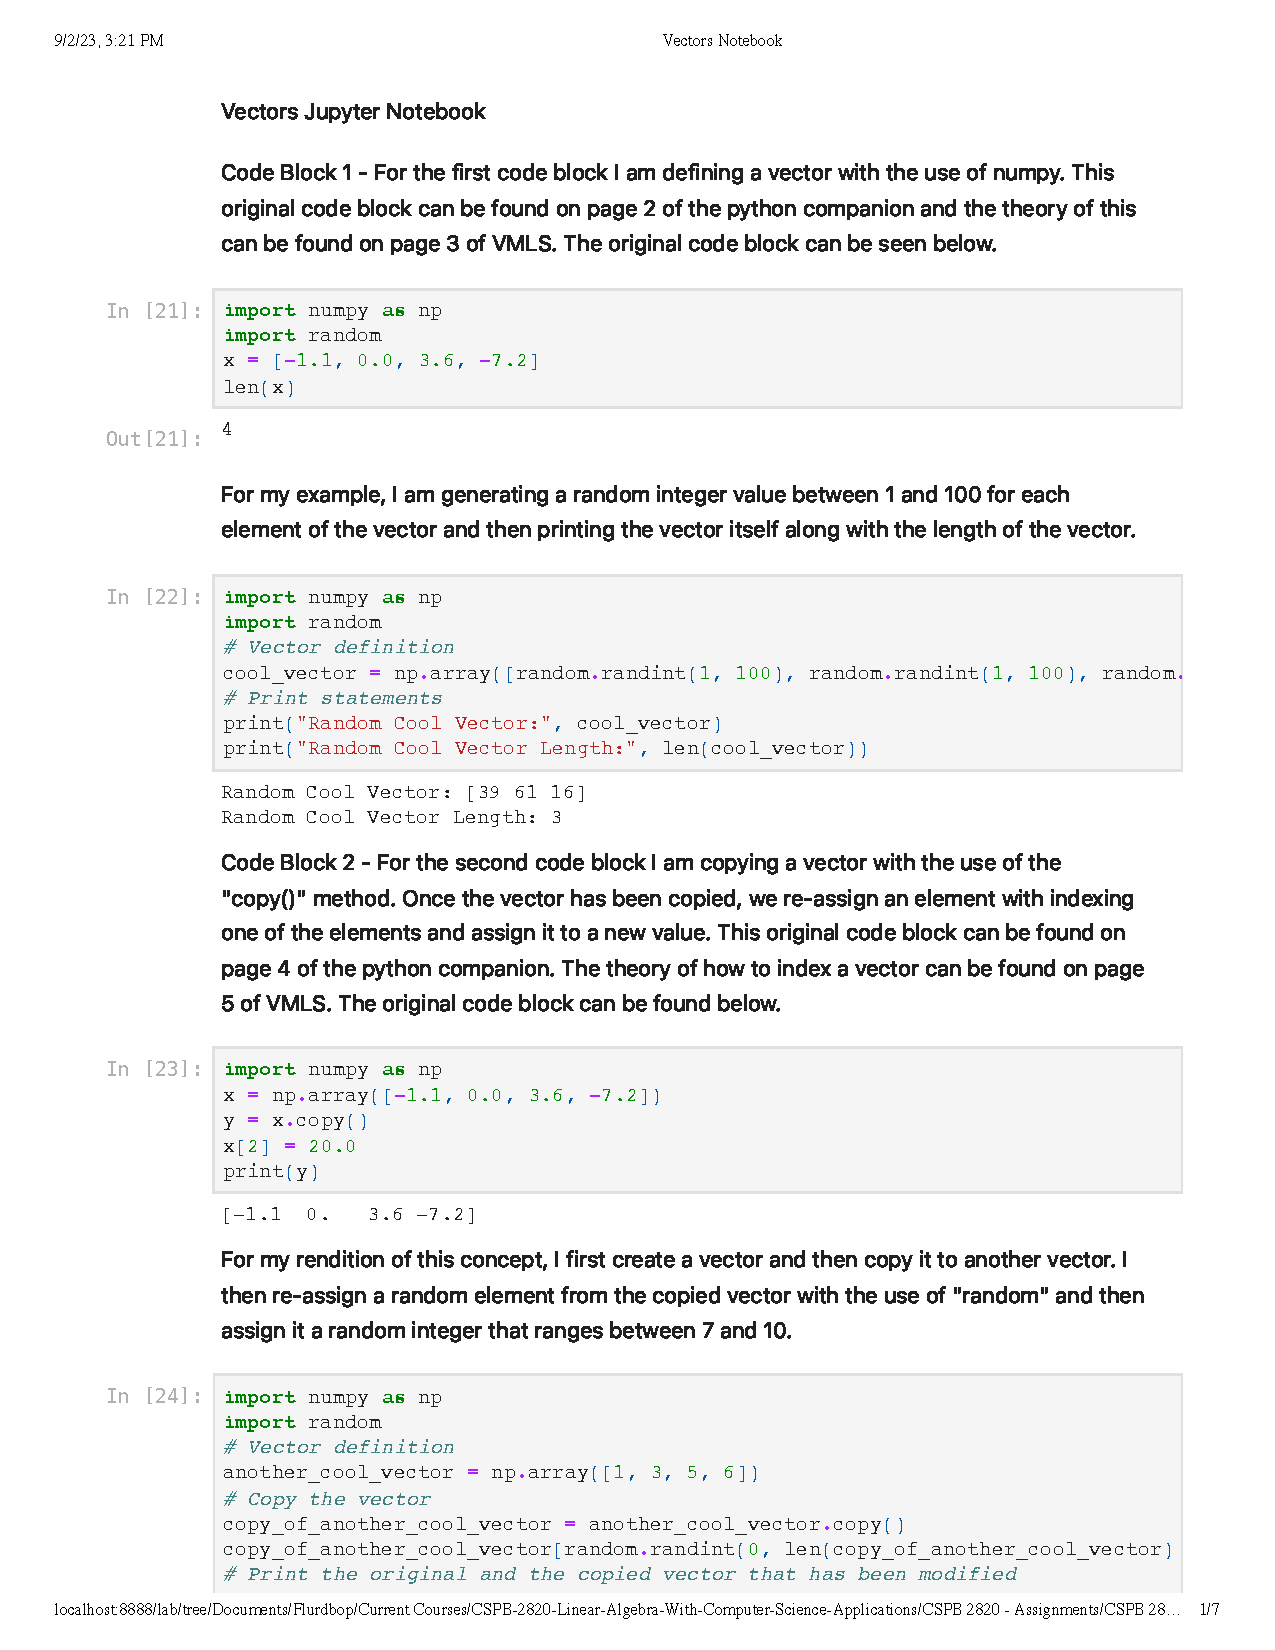
\includepdf[pages={-}, pagecommand={\thispagestyle{fancy}}, width=\paperwidth, offset=0 0]{./PDF/Notebook.pdf}
\end{problem}

% Problem 5 Summary
\begin{summary}{Problem 5 Summary}
    \begin{statement}{Procedure}
        \begin{itemize}
            \item For this problem we showcase different examples from VMLS with the use of a Jupyter notebook
        \end{itemize}
    \end{statement}
    \begin{statement}{Key Concepts}
        \begin{itemize}
            \item This problem showcases many properties of inner products with the use of Jupyter notebook and python
        \end{itemize}
    \end{statement}
    \begin{statement}{Variations}
        \begin{itemize}
            \item We could be asked to copy code from a different section of VMLS
        \end{itemize}
    \end{statement}
\end{summary}